\documentclass[conference]{IEEEtran}
\IEEEoverridecommandlockouts
% The preceding line is only needed to identify funding in the first footnote. If that is unneeded, please comment it out.
\usepackage{cite}
\usepackage{amsmath,amssymb,amsfonts}
\usepackage{algorithmic}
\usepackage{graphicx}
\usepackage{textcomp}
\usepackage{xcolor}
\usepackage[utf8]{inputenc}
\usepackage[hidelinks]{hyperref}
\def\BibTeX{{\rm B\kern-.05em{\sc i\kern-.025em b}\kern-.08em
    T\kern-.1667em\lower.7ex\hbox{E}\kern-.125emX}}
\begin{document}

\title{Road Accident Prediction in Time and Space}

\author{\IEEEauthorblockN{1\textsuperscript{st} Antoine Hébert}
\IEEEauthorblockA{\textit{Department of Computer Science and Software Engineering} \\
\textit{Concordia University}\\
Montréal, Québec, Canada \\
an\_heb@encs.concordia.ca}
\and
\IEEEauthorblockN{1\textsuperscript{st} Timothé Guédon}
\IEEEauthorblockA{\textit{Department of Computer Science and Software Engineering} \\
\textit{Concordia University}\\
Montréal, Québec, Canada \\
t\_guedon@encs.concordia.ca}
\and
\IEEEauthorblockN{3\textsuperscript{rd} Tristan Glatard}
\IEEEauthorblockA{\textit{Department of Computer Science and Software Engineering} \\
\textit{Concordia University}\\
Montréal, Québec, Canada \\
tglatard@encs.concordia.ca}
\and
\IEEEauthorblockN{4\textsuperscript{th} Brigitte Jaumard}
\IEEEauthorblockA{\textit{Department of Computer Science and Software Engineering} \\
\textit{Concordia University}\\
Montréal, Québec, Canada \\
bjaumard@cse.concordia.ca}}

\maketitle

\begin{abstract}
Road accidents are an important issue of our modern societies, responsible for millions of deaths and injuries.
In this paper we show how one can leverage open datasets from a city like Montreal, Canada, to create some accident prediction models, using state-of-the-art big data analytics methods.
Such models could then be used in the context of road accident prevention, but also to identify key factors that can lead to a road accident, and eventually, help to elaborate new policies.
This study also explains how we dealt with the severe class imbalance issue of the accident prediction problem, a recurrent issue that touches many other scientific domains like medical diagnoses or fraud detection.
In particular, we show how we implemented Balanced Random Forests, a variant of the Random Forests machine learning algorithm, into the Scala and Python APIs of Apache Spark big data framework.

\end{abstract}

\begin{IEEEkeywords}
machine learning, road accidents prediction
\end{IEEEkeywords}

\section{Introduction}
According to the World report on road traffic injury prevention, 2004, more than one million people die every year from car accidents and dozens of millions of people are being injured\cite{Peden2004}.
In this report, the World Health Organization also describe road traffic systems as “the most complex and the most dangerous system with which people have to deal every day”.
This issue is all the more important that the number of accidents is forecast to continue rising.
In the last decade, Big Data Analytics has been emerging \cite{Gandomi2015}, allowing scientists to handle a very large amount of data, but also complex and heterogeneous data, in order to extract useful insights from it.
In the context of accident prediction, Big Data Analytics could provide insights on the conditions leading to an increased risk of road accidents that could then be used to develop traffic-related policies and prevention operations.
Our contributions include: 
\begin{itemize}
\item a demonstration of how simple and easily available datasets can be fused to obtain meaningful features for road accident prediction,
\item the implementation of Balanced Random Forest introduced by Chen et al.\cite{Chen2004} in Apache Spark for efficient distributed training.
\item a comparison of three different machine learning algorithms dealing with data imbalance in the context of road accident prediction,
\item a real-time road accident prediction model for the island of Montreal with good performances
\end{itemize}
All the source code used is publicly available on Github under the MIT license. \footnote{https://github.com/GTimothee/accident-prediction-montreal}

\subsection{Need to be extended, some ideas:}

  As compared to previous studies we have a much bigger dataset of more than a hundred thousands accidents and while other recent studies predict the risk  of an accident in large space area of several thousands of square meter, we try to predict the occurrence of an accident in road segments of a few hundred meters. This lower resolution make the machine learning problem harder but also more useful, indeed knowing the accident risk is low in an area with very few roads is not helpful. 

The rest of this paper is organized as follows: section 2 presents the related work of this paper, the section 3 presents the datasets we used and how we fused them to create positive and negative examples for the road accident prediction, the section 4 presents how we performed the feature engineering, the feature selection and the hyper-parameter tuning, the section 5 present our results and the section 6 discusses them.

\section{Related work}
Accident prediction has been extensively studied in the last decades.
Historically, variations of the Poisson regression such as the negative binomial regression were used to predict the number of accidents which occurred on a given road segment, but during the last decade, machine learning algorithms have been used with success for accident prediction.
The features usually include information on the road such as the number of lanes, the average daily traffic, and the curvature, as well as weather information such as the average precipitation and the temperature.
In 2005, Chang \cite{Chang2005} compared the performances of a negative binomial regression with that of an Artificial Neural Network to predict the number of accidents during a year on a road segment from a major freeway in Taiwan.
The dataset used contained data from the years 1997 and 1998, which resulted in 1338 accidents.
The ANN achieved slightly better result, with an accuracy of $61.4\%$ on the test dataset.
On the same dataset, Chang et al.\cite{Chang2005b} also used decision trees for accident prediction in order to get more insights on the important variable for accident prediction.
It appears that the average daily traffic and the number of days with precipitation are the most useful features.
The decision tree reached an accuracy of $52.6\%$ on the test dataset.
Lin et al.
\cite{Lin2015} compared the performances of Frequent Pattern trees with that of random forests for feature selection.
They used k nearest neighbor and Bayesian networks for the real-time accident prediction on a segment of a highway.
Using the mean and sometimes the standard deviation of time series corresponding to the weather condition, the visibility, the traffic volume, the traffic speed, and the occupancy, their models predict the occurrence of an accident at the end of the time series.
They obtained the best result using the Frequent Pattern trees feature selection and achieved an accuracy of $61.7\%$.
We note that they used a small sample of the possible negative examples.
Theofilatos\cite{Theofilatos2017} also used real-time data on two urban arterials of the city of Athens to study road accident likelihood and severity.
Random Forests were used for feature selection and a Bayesian logistic regression for accident likelihood prediction.
The most important features identified were the coefficient of variation of the flow per lane, the speed and the occupancy, and the standard deviation of the speed and the occupancy.
In addition, many publications aim at predicting the severity of an accident using various information from the accident in order to understand what causes an accident to be fatal.
Chong et al.\cite{Chong2005} used decision trees, neural network and a hybrid model using a decision tree and a neural network.
They obtained the best performances with the hybrid model which reached an accuracy of $90\%$ for the prediction of fatal injuries.
They identified that the seat belt usage, the light conditions and the alcohol usage of the driver are the most important features.
Abellán et al. \cite{Abellan2013} also studied traffic accident severity by looking at the decision rules of a decision tree using a dataset of 1801 highway accidents.
They found that the type and cause of the accident the light condition, the sex of the driver and the weather were the most important features.

All of these studies use relatively small datasets using data from only a few years or only a few roads.
Indeed, it can be hard to collect all the necessary information to perform road accident prediction on a larger scale, and dealing with big datasets is more difficult.
However, more recent studies performed accident prediction at a much larger scale, usually using deep learning models.
Deep learning models can be trained online so that the whole dataset does not need to stay in memory.
This makes it easier to deal with big datasets.

Chen et al. \cite{QChen2016} used human mobility information coming from mobile phone GPS data and historical accident records to build a model for real-time prediction of traffic accident risk in areas of 500 by 500 meters.
The risk level of an area is defined as the sum of the severity of accidents that occurred in the area during the hour.
Their model achieves an RMSE of $1.0$.
They compared the performance of their deep learning model with the performances of some of the classical machine learning algorithms: a Decision Tree, a Logistic Regression and a Support Vector Machine (SVM), which all got worse performances of respectively $1.41$, $1.41$ and $1.73$ for the RMSE.
We note that they have not tried the random forest algorithm which usually has good prediction performances.
Najjar et al. \cite{Najjar2017}, trained a convolutional neural network using historical accident data and satellite images to predict the risk of accidents on an intersection using the satellite image of the intersection.
Their best model reaches an accuracy of $73\%$.
Yuan et al. \cite{Yuan2018} used an ensemble of Convolutional Long Short-Term Memory (LSTM) neural networks for road accident prediction on the state of Iowa.
Each neural network of the ensemble is predicting on a different spatial zone so that each neural network learns the patterns corresponding to its zone, which might be a rural zone with highways or an urban zone.
They used a high-resolution rainfall dataset, a weather dataset, a road network dataset, a satellite image and the data from traffic cameras.
Their model reaches an RMSE of $0.116$ for the prediction of the number accident during a day in an area of 25 square kilometers.

These more recent studies are particularly interesting because they achieve good results for the prediction of road accidents in time and space in larger areas than previous studies who focused on a few roads. But unlike previous studies, they only provide an estimation of the risk of accidents for large areas. In our study, we decided to focus on urban accidents prediction by focusing on the island of Montreal, but with much higher prediction resolution. We used a time resolution of one hour and a spatial resolution of road segments delimited by the road intersections. The road segments used have an average length of 124 meters, $82\%$ of the road segments are less than 200 meters long.

\subsection{Related work on data imbalance ?}

\section{Datasets fusing}
\subsection{Datasets}
We used three public datasets provided by the city of Montreal and the government of Canada: 
\begin{itemize}
\item Montreal Vehicle Collision: This dataset provided by the city of Montreal contains all the road collisions reported by the police occurring from 2012 to 2018 on the island of Montreal.
For each accident, the dataset contains the date and localization of the accident, information on the number of injuries and death, the number of vehicles involved, and information on the road condition.
We used only the localization and the date of the accident since we do not have the other piece of information when no accident happened.
Another dataset with all vehicle collision in Canada is available but without the localization of the accident, therefore we restrained our analysis to the city of Montreal.
\item National Road Network: This dataset provided by the government of Canada contains the geometry of all roads in Canada.
For each road segment, a few meta-data are given.
For roads in Quebec, the speed limit and the surface type are not provided.
The data was available in various format, we chose to use the Keyhole Markup Language, which is a standard of the Open Geospatial Consortium since 2008.
This format is based on the Extensible Markup Language (XML), which make it easier to read using existing implementation of XML parsers. From this dataset, we selected $44111$ road segments belonging to the island of Montreal.

\item Data Historical Climate Data: This dataset provided by the government of Canada contains hourly weather information measured at different weather stations across Canada.
For each station and every hour, the dataset provides the temperature, the humidity, the wind direction and speed, the visibility, the atmospheric pressure and observations of atmospheric phenomenon such as snow, fog, rain, etc.
\end{itemize}

\subsection{Positive and negative examples generation}
This machine learning problem can be stated as a binary classification problem, the positive class is the occurrence of an accident and the negative class is the non-occurrence of an accident on a given road at a given date and hour.
The vehicle collision dataset contains 150 thousands of collisions, among them $134 489$ contain the date, the hour and the localization of the accident.
For each of these accidents, we identify the closest road segment.
These pairs of a time and a road segment are used as positive examples.
For the negative examples, we generated a random sample of 2 millions combinations of time and road segment which did not appear in the collision dataset.
 The generation of these examples together with the join operation with the data from the other datasets made our dataset generation heavy. We used the big data framework Apache Spark to implement these dataset fusing operations. The dataframe API is particularly adequate for this kind of operation.
Still our first implementation add impractical time and memory space requirements to generate the dataset.
It was querying the Historical Climate Data API in real-time with a cache mechanism.
Our idea was to collect only the weather stations and hours necessary for our sample of negative examples, but it resulted in bad performances.
We got a performance increase by first building a Spark dataframe with all the Historical Climate Data for weather stations around Montreal and then joining the two datasets.
We conducted a detailed analysis of our algorithm to improve its performances.
We notably obtained a good performance increase by not persisting intermediary results of the road segment identification for accidents.
As opposed to what we initially thought, recomputing these results was faster than writing and reading them in the cache.
Finally, the identification of the road segment corresponding to accidents was very memory intensive, we modified this step to be executed by batch of one month.
 With these improvements and a few other tricks including partitioning the data frame at key points in our algorithm, we managed to reduce the processing time to a reasonable time.
We also used a cluster from “Compute Canada” to take maximum advantage of Apache Spark distributed nature for the generation of examples and the hyper-parameter tuning of our models.


\section{Model development}

\subsection{Algorithms selected}
For this study, we chose to focus on tree-based algorithms because they have proven their efficiency compared to classical statistical methods and allow for easier interpretability than deep learning algorithms.
In particular, we implemented the Balanced Random Forests (BRF) algorithm in Apache Spark to deal with class imbalance which is a prominent issue in road accident prediction.
To validate the performance of our version, we run an experiment with a simple synthetic dataset to compare its performances with the standard implementation of Random Forest (RF) in Spark using random under-sampling of the majority class.
As expected, Balanced Random Forest performed better.
Balanced Random Forests in one of the two methods proposed by Chen, Liaw, and Breiman\cite{Chen2004} to deal with class imbalance when using Random Forest.
Balanced Random Forests are like Random Forests, but with a difference during the bootstrapping phase, for each tree of the forest, a random under-sampling of the majority class is performed in order to obtain a balanced sample.
Intuitively, Balance Random Forest is an adaptation of random under-sampling of the majority class making use of the fact that Random Forests are an ensemble method.
Random under-sampling usually performs better than more advanced methods like SMOTE or NearMiss \cite{Branco2016}.
Chen, Liaw and Breiman\cite{Chen2004} also proposed in the same paper, the Weighted Random Forest (WRF) which consists in giving more weight to the minority class at the building time of each tree and during the measure of the gain in impurity and during the class prediction of each terminal node.
While neither method is clearly better than the other in terms of prediction power, we chose BRF because it is found to be more computationally efficient (because of the under-sampling).
Interestingly, Wallace et al. \cite{Wallace2011} presents a theoretical analysis of the data imbalance problem and suggest to use methods like Balance Random Forest.

We decided to compare the performance of the Balanced Random Forests algorithm with the performances of one of the very efficient implementations of Gradient Boosted Trees: XGBoost which offers parameters to deal with data imbalance as well.

\subsection{Implementation of balanced random forest in Apache Spark}
The Balanced Random Forests algorithm was not implemented in Apache Spark.
An implementation is available in the python library imbalanced-learn\cite{imbalance} which implements many algorithms to deal with data imbalance using an API inspired by scikit-learn, but the size of our dataset made it impossible for us to use this library.
Therefore, we implemented Balance Random Forests in Apache Spark.

In the Apache Spark implementation of Random Forests, the bootstrap step is made before starting to grow any tree.
For each sample, an array contains the number of time it will appear in each tree.
When doing sampling with replacement, each value of this array is given by a Poisson distribution.
The parameter of the Poisson distribution corresponds to the sub-sampling rate hyper-parameter of the Random Forest, which specifies the size of the sample used for training each tree as a fraction of the total size of the dataset.
Indeed, if for example we want each tree to use a sample of the same size of the whole dataset, the sub-sampling ratio will be set to 1.0, which is indeed the number of time a given example will appear in a tree on average.

In order to implement Balanced Random Forests, we modified the parameter of the Poisson distribution to use the class weight multiplied by the sub-sampling ratio, this way a negative sample with for example the weight 0.25 has 4 times less chance to be chosen to appear in a given tree.
This implementation has the advantage that it did not require a big code change and will be easy to test, but it also has a disadvantage, users probably expect linearly correlated weight to be equivalent, which is not the case in our implementation.
	
In order to be compatible with other possible use cases, the weights are actually applied per samples and not per class.
This is a choice made by Apache Spark developers that we respected.
In order to support sample weights, we create a new Poisson distribution for each sample.
To make sure the random number generator is not reseeded for each sample, we use the same underlying random number generator for all Poisson distributions, this also helps reduce the cost of creating a new Poisson distribution object.
Like with other estimators accepting weights, our Balanced Random Forests implementation use weight from a weight column in the samples data frame.
We adapted the Python wrapper of the random forest classifier to accept and forward weights to the algorithm in Scala.
Finally, we did a first validation of our implementation using an artificially generated imbalanced dataset and compared the results of both standard random forest and BRF.
While BRF had better results in terms of area under PR (which was our selected measure) (98.\% against 98.1\%), the standard random forest had better F1 score (99.7\% against 98.8\%) with default threshold.
This emphasized that we were right in our choice of the area under PR curve as our measure in the case of class imbalance, indeed with a good threshold, the BRF model performs better.

\subsection{Feature Engineering}
For each example corresponding to a date, an hour, and a road segment we computed features that can be helpful for road accident prediction using the datasets we had collected. We created three types of features, weather features, features from the road segment and features from the date and time.

For the weather features, we used data from the Historical Climate Dataset.
In order to estimate the weather information at the position of the road segment, we use the mean of the weather information from all the surrounding weather stations at the date and hour of the example weighted by the inverse of the square of the distance between the station and the road segment.
We initially used the inverse of the distance, but we obtained a small improvement in performances when squaring the inverse of the distance.
It makes sense since the weather information is probably much closer to the closest stations than the other ones.
We tried higher power, but the results were not as good.
It could be interesting to experiment with different power values for each weather information.
We used all the weather information provided by the Historical Climate Dataset.
The features are: the temperature, the dew point temperature which is a measure of the humidity, the real humidity percentage, the wind direction, the wind speed, the visibility, the atmospheric pressure, the Hmdx index, which is a measure of felt temperature and the wind chill which is another measure of the felt temperature using the wind information.
In addition, the historical weather dataset, provide a multi-label categorical variable providing the observations of atmospheric phenomenon such as snow, fog, rain, etc.
We used this last variable to create a binary variable that we called risky weather which is true when the following phenomenons are observed: Freezing Rain, Freezing Drizzle, Snow, Snow Grains, Ice Crystals, Ice Pellets, Ice Pellet Showers, Snow Showers, Snow Pellets, Ice Fog, Blowing Snow, Freezing Fog.

For the features from the road segments, we were limited by the limited metadata provided on the road segments.
From the shape of the road segment, we computed the length of the road segment, and from the name of the street, we identified the type of road (Highway, street, boulevard, etc.).
In addition, road segments are classified into three different levels in the dataset depending on their importance in the road network, we created a categorical feature from this information.
For these two categorical features, we encoded them as suggested in The Elements of Statistical Learning\cite{elementsofstat} in section 9.2.4, instead of using one hot encoding which would create an exponential number of splits, we index the categorical variable ordered by the proportion of the examples belonging to the given category which are positive samples.
This encoding guarantee to provide optimal splits on these categorical variables.
Lastly, we added a feature giving the number of accidents which occurred previously on this road segment.

For the date features, we took the day of the year, the hour of the day, and the day of the week.
We decided to make the features day of the year and hour of the day cyclic.
Indeed, for example with the feature hour of the day, 23 hour is very close to 1 hour, but in the usual encoding, this does not appear to the machine learning algorithm.
With cyclical encoding, we compute two features, the first one is the cosine of the original feature scaled between 0 and two pi, and the second one is the sine of the original feature scaled between 0 and two pi.
In this form, the hours 23 and 1 appear close.
In addition to these basic date features, we computed an approximation of the solar elevation using the hour of the day, the day of the year and the GPS coordinates. The solar elevation is the angle between the horizon and the sun. 

\subsection{Choice of an evaluation metric}
Usually, the accuracy is used to evaluate the performance of classification models, but with an imbalance dataset, this measure does not reflect the real predictive power of the model.
Indeed, it is usually easy to predict that an example is in the negative class and machine learning models will usually achieve a very good accuracy for the negative class.
Since most examples belong to the negative class, the overall accuracy will be very good as well.
However, what we are usually interested in, and this is the case in accident prediction, is to correctly detect the positive examples.
Therefore, we used the precision and the recall measures.
The precision is the proportion of examples detected as positive which are actually positive and the recall, also called the true positive rate, is the proportion of positive examples which are detected as positive.
The false positive rate (FPR) is also usually used in binary classification, it is the proportion of negative examples which are detected as positives.
With an imbalance dataset, the FPR will usually stay very low because the number of negative is high, that is why we used the precision instead.
By decreasing the threshold used by the machine learning model to consider an example as positive, we can get a better recall with a worse precision, in order to measure the predictive power of our model independently of the choice of the threshold, we used the area under the precision-recall curve as our main metric.

\subsection{Identifying the most important features}
Random forests allow to measure feature importances by computing the total decrease in impurity of all splits using the variable weighted by the number of samples.
This variable importance measure is not perfect for interpretability since it is biased toward non-correlated variables, but it helps to select the most useful features for the prediction.
With a feature importance of $70\%$, the number of accidents which occurred on the road segment during the previous years is clearly the most useful feature, which is not surprising.
The figure \ref{feature importances} presents the importances of the other features as reported by the Balanced Random Forest algorithm.
As we can see, the next important features are the cosinus of the hour of the day, which probably separate day from night, the length of the road segment, and its importance.
Then comes the position of the road segment, the sinus of the hour of the day and the solar elevation. Finally comes the weather features with the visibility first.
We believe the weather features have lower importances because they are strongly correlated. 
The gain in impurity obtained with the information they contain is distributed over all the correlated features.
Surprisingly, the day of the year and the risky weather features have a significantly lower feature importance. 
We believe the visibility, the atmospheric pressure and the humidity contains their information in a more efficient way.
As compared to the count of accident feature the other features seem to have almost no importance, but the performances of the model decrease significantly if we remove one of them.
We removed the features wind direction, wind speed, dew point temperature, wind chill, hmdx index and day of month, since they had much lower feature importances. The wind and the day of month apparently are not linked with the probability of a road accident to occur.


\begin{figure}[htbp]
\centerline{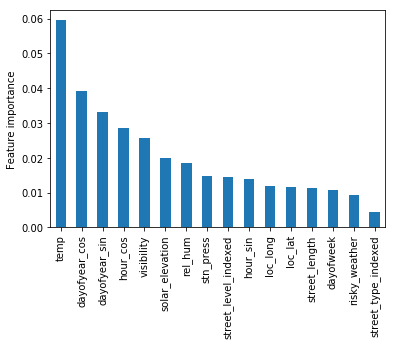
\includegraphics[height=7cm, keepaspectratio]{figures/brf_fi_nocount.png}}
\caption{Feature importances computed by the Balanced Random Forest excluding the accident count feature}
\label{feature importances}
\end{figure}

\subsection{Hyper-parameter tuning}
In order to determine the optimal hyper-parameter, we first performed automatic hyper-parameter tuning using Apache Spark ML library grid search using cross-validation.
Because the training on the whole dataset would have been too high, we took a small sample of the dataset.
Still, We could not test many parameters combination using this method.

Once we got a first tuning result with grid search we continued manually by following a plan, do , check, adjust method, using the measure of the area under the precision-recall curve, the precision and recall with different threshold on the test set and the training set we were able to better understand how the performances of our model could be improved.

Interestingly, despite using many trees, our Random Forest algorithms tended to over-fit very quickly as soon as the maximum depth parameter goes above 18.
We eventually used only 100 trees, because adding more trees did not increase performances.
We have not tried more than 200 trees, maybe many more trees would have been necessary to increase the maximum depth without over-fitting, but then the training time would not be reasonable.

\section{Results}
These results have been obtained by training the algorithms on the whole dataset of positive samples and with a sub-sample of $0.05\%$ of the 2 billion possible negative examples. This corresponds to a total of 1.3 million examples with a data imbalance reduced to a factor of 8.
To evaluate this model we used a test set containing the last two years of our dataset, the model is trained on the 4 previous years and use only data from these years.
For example, the "count\_accident" feature contains only the count of accidents occurring from 2012 to 2016 on the road segment.

The following table presents the results we obtained with the classical random forest algorithm with random under-sampling, and with the Balanced Random Forest algorithm:

\begin{table}[htbp]
\caption{Results Summary}
\begin{center}
\begin{tabular}{|l|l|r|r|r|}
\hline
          & \textbf{Algorithm} &     BRF &      RF &     URF \\
\hline
\textbf{Test set} & \textbf{Accuracy} &  0.8146 &  0.9170 &  0.8079 \\
          & \textbf{Area under PR curve} &  0.5544 &  0.5575 &  0.5516 \\
          & \textbf{Area under ROC curve} &  0.8873 &  0.8915 &  0.8406 \\
          & \textbf{F1 score} &  0.8454 &  0.9070 &  0.8454 \\
\hline
\textbf{Train set} & \textbf{Accuracy} &  0.8292 &  0.9294 &  0.8829 \\
          & \textbf{Area under PR curve} &  0.6623 &  0.7272 &  0.9529 \\
          & \textbf{Area under ROC curve} &  0.9417 &  0.9485 &  0.9570 \\
          & \textbf{F1 score} &  0.8564 &  0.9221 &  0.8827 \\
\hline
\end{tabular}
\label{result summary}
\end{center}
\end{table}

We obtain the following precision recall curves created by computing the precision and the recall metrics when varying the threshold used by the model.

\begin{figure}[htbp]
\centerline{\includegraphics[height=6cm, keepaspectratio]{figures/pr_brf_and_rf.png}}
\caption{Precision as a function of the recall}
\label{precision recall rf}
\end{figure}

As we can see, the balanced random forest performs almost as good as the random forest after random under-sampling of the majority class. These models can achieve a recall of $82\%$ with a precision of $33\%$.

\section{Discussion}
The overall results are good but mostly rely on the count of previous accidents on the road segment.
This is not an issue for accident prediction, but it does not help to understand why these roads are particularly dangerous.
We believe one of the reason why this features is extremely useful is that we do not have information about the average traffic volume for each road, in addition to the dangerousness of a road segment, this feature carries the information of the number of vehicles using the road.
Accident prediction is a very hard machine learning problem because even if the risk is very high for an accident to occur, and even if an accident almost occur, the by reacting quickly, the driver can manage to avoid it although the conditions were almost exactly the same as when an accident occurs.
We would need information on the state of the drivers and the state of the vehicle to significantly improve performances.

As opposed to what we would have expected, the Balance Random Forest did not obtained much better performances than the Random Forests with random under-sampling.
We believe this is caused by the fact that negative examples are not that different from each other and the information they contains is well captured by a single random sub-sample.
We can notice, that the Balance Random Forest does not over-fit as much as the Random Forest algorithm.

We can see that the most important variables are the features of the road segment.
We believe better performances could be reached by providing more context information on where the road is located. However, even with more features and more data, it is very difficult to achieve very good performances because of the nature of the problem.

We can see that as we discussed previously the accuracy is not a good metric for the evaluation of the performances of a classification model with data imbalance. Indeed, although we obtain a very good accuracy of $83\%$, we detect only $82\%$ of accidents with a precision of $33\%$. If we had used a bigger sample of negative examples, we would have had an even better accuracy since most negative examples are easy to classify.

also practical example of what our prediction results means.

\subsection{Future work}
We believe better performances could be reached by adding more features from other datasets.
For the city of Montreal, we identified two particularly interesting datasets: a dataset with the location and dates of construction work on roads, and a dataset with the population density.
These datasets might not be as easily available for over areas, but for Montreal, they could improve performances.
This accident prediction model can be used directly to know on which road segments accidents are the most likely to happen in a given hour in order to take measure to reduce risk.
This would require to put this model into production.
The historical climate dataset, would have to be replaced by a weather forecast dataset.
The most important feature is the number of accidents which happened during the previous year, while this feature help a lot to reach useful prediction performances, it does not help in understanding the characteristics of a road segment which makes it dangerous.
A human analysis of these particularly risky road segment could detect patterns that could help to take measure to reduce the number of accidents in Montreal.
This can also allow to improve our current accident prediction model, if the detected patterns can be used by fusing other datasets.

\section*{Acknowledgment}

The authors would like to acknowledge Compute Canada for providing access to the computation cluster.

\bibliographystyle{IEEEtran}
\bibliography{biblio}

\end{document}